% !Mode:: "TeX:UTF-8:Main"
\makeatletter
\def\UlrikeFischer@package@version{0.51}
\def\UlrikeFischer@package@date{2021-03-07}
\makeatother
\RequirePackage{pdfmanagement-testphase}
\DeclareDocumentMetadata{pdfversion=1.7,lang=en-UK, uncompress}

\documentclass[DIV=12,parskip=half-,bibliography=totoc]{scrartcl}
\usepackage{scrlayer-scrpage}
\usepackage{fontspec}
\setmainfont{Heuristica}
\usepackage{unicode-math}
\usepackage[english]{babel}
\usepackage[autostyle]{csquotes}
\usepackage{microtype}
\usepackage{listings}
\def\lstlanguagefiles
    {lstlang0.sty,lstlang1.sty,lstlang2.sty,lstlang3.sty}

\lstset{basicstyle=\ttfamily, columns=fullflexible,language=[LaTeX]TeX,
        escapechar=*,
        commentstyle=\color{green!50!black}\bfseries}
\usepackage[pdfdisplaydoctitle=true,hyperfootnotes=false]{hyperref}
\hypersetup{pdftitle=The newpax package,pdfauthor=Ulrike Fischer}
\usepackage{ydoc-desc}

\usepackage{newpax}
\directlua{require("newpax")}
% write pax and .newpax files
\directlua
  {
    newpax.writenewpax("doc-input1")
    newpax.writenewpax("doc-input2")
    newpax.writepax("doc-input1")
    newpax.writepax("doc-input2")
  }
\newpaxsetup{usefileattributes}

\title{The \pkg{newpax} package, v\csname UlrikeFischer@package@version\endcsname}
\subtitle{Reinserting annotations from included pdf file}
\date{\csname UlrikeFischer@package@date\endcsname}
\author{Ulrike Fischer\thanks{fischer@troubleshooting-tex.de}}

\begin{document}
\maketitle

\section{Introduction}

Links in a PDF are created with annotation objects. Such an object is not connected to the content
or text, but simply describes an (rectangular) area on the page and defines an action if the
cursor is in the area. The coordinates of the area are given in absolute page coordinates.
The action of such an annotation can be an external URL, but also an internal destination.
Such destination are objects describing a page and some instructions how to display the page---again using absolute coordinates.

When a PDF is included in another PDF---may it be with \cs{includegraphics} or with \cs{includepdf}--the annotation coordinates no longer make sense as they don't refer to the receiving page (and often the action of an annotation doesn't make sense either), so all TeX-engines and backends strip them away when including a PDF: the net effect is that external and internal links are lost.

The \pkg{pax} package from Heiko Oberdiek offers a solution for this problem: it extracts all the annotations
and destinations of the included PDF in a text file, does some clever recalculations of their coordinates and reinserts them.
The package works basically fine but has a few drawbacks: To collect the annotation one has to run an external
java program which relies on an now outdated library, and it works only with pdf\LaTeX{}.

The \pkg{newpax} tries to address these problems. It offers a lua script to extract the annotations.
The script can be used with lua(la)tex  and no external tools are needed. The annotations can
then be reinserted either with the \pkg{pax.sty} or with the new \pkg{newpax.sty} whose code based in large parts on the \pkg{pax} package: it uses its data structure and the original code to calculate the coordinates (with a few minor bug corrections), but the pdf\LaTeX{} primitives have been replaced by commands from the new \LaTeX{} PDF management in \pkg{pdfmanagement-testphase} so it should works with all major engines and backends (with the exception of dvips).


\section{Quick use instructions}

\subsection{Step 1: extract and collect the annotations}

The lua script offers a function which take as argument the name of a PDF (without the extension).
The function can be used in some lua scripts but also in a document which then must be compiled
with lualatex.

\lstinputlisting[caption=doc-extract-newpax.tex]{doc-extract-newpax.tex}

Running this document will create the files \file{doc-input1.newpax} and \file{doc-input2.newpax}.

To find the graphics \texttt{kpathsea} is used. This means that graphics in texmf trees will work and
you can also use paths to directories, but settings in \cs{graphicspath} are ignored. The newpax
file is currently written into the current directory, which means that graphics with the same name
in different locations won't work easily (with lualatex you could create the newpax file in the document
just before it is needed). Later versions of the package will probably add some options for this case,
but for now use at best distinct file names.


\subsection{Step 2: Using the \texttt{.newpax}-file with \texorpdfstring{\pkg{newpax}}{newpax}}

The package \pkg{newpax} is based on the package \pkg{pax} but extends it in various way.
It is still an experimental package, and it requires the new \LaTeX{} PDF management
code in \pkg{pdfmanagement-testphase} package. This new code is---as the name implies---currently in the testphase and \emph{not} compatible with every package!

The following listing shows how to use \pkg{newpax}.

\begin{itemize}
\item It should work with pdflatex, lualatex and xelatex. The latex/dvips route fails as this can't include PDF anyway.
\item Some provision have been added to allow multiple inclusion of the same PDF, but if you insert different sets of pages from a PDF some destinations can still be missing. So better avoid it.
\item You can choose for every file if border color and styles of links are taken from the source PDF or from the hyperref settings. But you can't adjust or change colored links.
\item You can add additional settings to the annotations, for example an \texttt{/F} flag, with

\begin{lstlisting}
\ExplSyntaxOn
\pdfannot_dict_put:nnn {link/URI}{F}{4}
\ExplSyntaxOff
\end{lstlisting}

\end{itemize}

\lstinputlisting[firstline=2,caption=doc-use-newpax.tex]{doc-use-newpax.tex}

\subsection{Combining the steps}

When using lualatex both step can be simply in the same document.
With other engines you can use \pkg{ifluatex}.



\section{Setup options}

\DescribeMacro\newpaxsetup{key-val option list}

This command allows to change the behaviour inclusion. It knows the following keys:

\begin{description}
  \item[\PrintKeyName{usefileattributes}] This is a boolean key. If set to true, the reinserted annotations will use the linkborder settings (color and style) of the included file, if set to false, the settings of the receiving PDF will take precendence.

  \item[\PrintKeyName{destsuffix}] This allows to add a suffix to the destination names. This is needed if a file with destinations
  is included more than once, to avoid to get multiple destinations.

 \item[\PrintKeyName{addannots}] This is a boolean key. It allows to switch on and off the reinserting of the annotations. When set to false  it also suppress warnings in the log if the \file{.newpax} file is not found.
     It is recommended to set it to false for graphics which don't have links.

\end{description}


\section{More Background}

Clickable links in a PDF are one example of an annotation. Annotations are areas on a page which are associated with an action. A typical annotation object could look like this in the PDF:

\begin{lstlisting}
15 0 obj
<<
/Type /Annot
/Subtype/Link
/Rect [147.716 654.025 301.887 665.15]
/Border[0 0 1]/BS<</S/U/W 1>>/H/I/C[0 1 1]
/A<</Type/Action/S/URI/URI(https://www.latex-project.org)>>
>>
endobj
\end{lstlisting}
This is an object of type \texttt{Annot} and subtype \texttt{Link}.
The \texttt{/Rect} value describes the rectangle of this annotation. The coordinates are absolute coordinates related to the current page. It is important to understand that an annotation is not connected to some page content but only to a location!
The \texttt{/Border} setting and the other values in this line describe the look and color of annotation. The \texttt{/A} value contains the action, in this case it is an url to an external website.


To \enquote{reactivate} the annotations of an included pdf one has to do a number of tasks.
\begin{itemize}
\item One must \emph{retrieve and store} the annotations of the included pdf. For links to external url's this requires to find only one object like the one shown above. But e.g. internal links point to destination objects and these must be found too.
\item One must \emph{recalculate} the rectangle coordinates to fit to the coordinate system of the target page: as the included pdf can be placed at various positions, scaled, rotated and even clipped this is not an easy task. Destinations have rectangles too that must be recalculated.
\item  One must  \emph{reinsert} the annotation and related objects. This has to take into account that a pdf is perhaps not included completely, a link shouldn't point to a missing page or a clipped annotation. It also has to take into account that a pdf is perhaps inserted more than once or in steps.
\end{itemize}

\subsection{Retrieving and storing annotations}

Theoretically one can do it manually: Uncompress the PDF (or when using \LaTeX, create directly an uncompressed one), open it in an editor and copy and paste all needed objects. Practically one naturally want some tool.

The \pkg{pax} package from Heiko Oberdiek consists of a perl script and a java-jar file \texttt{PDFAnnotExtractor} which can extract the necessary objects. It writes the information to a file with the extension \texttt{pax}.
When it has been successfully installed it works quite fine. Problems with this approach are
\begin{itemize}
\item \texttt{PDFAnnotExtractor} requires an external, old version of the java library of PDFbox which must be installed manually;
\item it requires a java installation and
\item it is not extensible.
\end{itemize}

The \pkg{newpax} package comes with a lua-file. It uses the \texttt{pdfe} library embedded in luatex to extract the annotations and other needed information. \pkg{newpax} writes the information to a file with the extension \texttt{pax} or \texttt{newpax}. The content of the files is (nearly) identical to the content of the \file{pax}-file written by \texttt{PDFAnnotExtractor}. The lua code was written by looking at example outputs from \texttt{PDFAnnotExtractor} and reproducing it in lua. The ordering of some elements is a bit different and some strings are output in a different way but for the examples I used the resulting \texttt{pax}-files can be used together with the original \texttt{pax.sty}. But due to the fact that the code was written without real spec simply by looking at examples, it is quite probably that the lua code is not yet handling all objects or options that \texttt{PDFAnnotExtractor} outputs.  But the code can rather easily be extended when the needs arises.

The code also doesn't handle structure elements, neither at the export nor at the import. I have yet no real idea what would be sensible here (and I'm quite sure that \texttt{PDFAnnotExtractor}  doesn't handle this either.)


\section{Importing annotations}

The \pkg{pax} package from Heiko Oberdiek does the hard work to recalculate the annotation rectangles and to decide which annotation and which destination should be reinserted. It also patches the \cs{includegraphics} command to automate this.
\pkg{newpax} reuses the core commands of \pkg{pax}. It only adds a number of switches and changes primitive to support more engines and backends.



\section{Example input}

\fbox{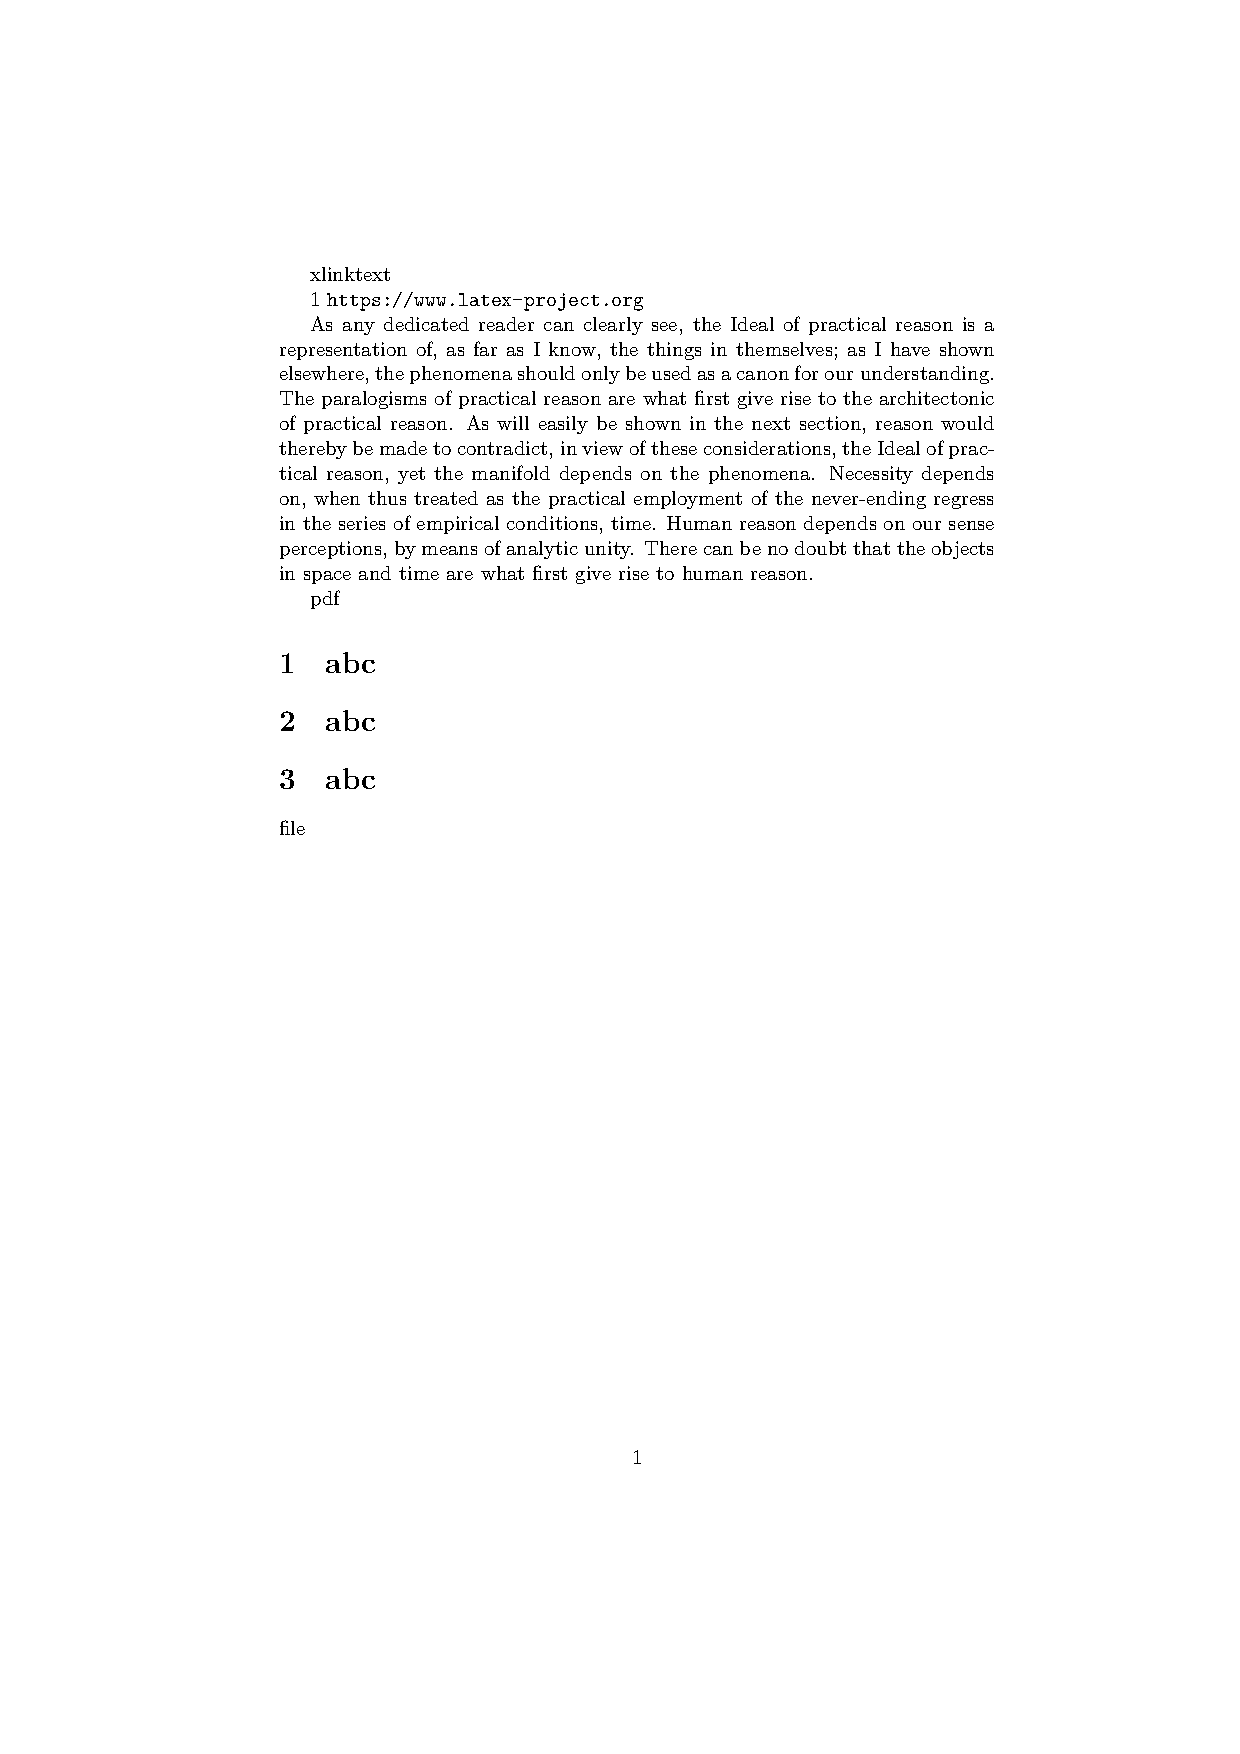
\includegraphics[scale=0.5,trim=4cm 15cm 8cm 3cm,clip,page=1]{doc-input1}}
\fbox{\includegraphics[scale=0.5,trim=5cm 15cm 8cm 3cm,clip,page=2]{doc-input1}}

Check also the output of the listing above, \file{doc-use-newpax.pdf}.

\section{Support for the \texorpdfstring{\pkg{pax}}{pax} package}

\subsection{Step 1: Extracting the annotations}
The lua script is also able to write \texttt{pax} files for the \pkg{pax} package (and so can be used to replace the java application).

For this extract the annotations like this:

\lstinputlisting[caption=doc-extract-pax.tex]{doc-extract-pax.tex}

\subsection{Step 2: Using the \texttt{.pax}-file with \pkg{pax.sty}}

Ensure that the \texttt{.pax} file created in step 1 can be found by your main document. You can then insert your PDF files together with their annotations like in the following listing.

\begin{itemize}
\item This works with pdflatex and lualatex. lualatex needs the extra code demonstrated in the document.
\item It needs two or three compilations until every reference is correct.
\item There is a small typo in \pkg{pax.sty} which affects clipping, the patch shown in the listing correct this.
\item Don't include PDFs with destinations twice as this will lead to duplicate destinations and pdflatex will complain.
\item If annotations should not be reinserted remove the \texttt{.pax}-file.
\item If \pkg{hyperref} is loaded you can change the color and style of link borders with hyperref options.
\end{itemize}

\lstinputlisting[firstline=2,caption=doc-use-pax.tex]{doc-use-pax.tex}

\end{document}
